\documentclass[12pt]{article} % use larger type; default would be 10pt
\usepackage[czech]{babel}
\usepackage[utf8]{inputenc} % set input encoding (not needed with XeLaTeX)

%%% PAGE DIMENSIONS
\usepackage{geometry} % to change the page dimensions
% \usepackage[left=2cm,right=2cm,top=2cm,bottom=2cm]{geometry}
\geometry{a4paper}
% \geometry{margin=2in} % for example, change the margins to 2 inches all round
% \geometry{landscape} % set up the page for landscape

\usepackage{graphicx} % support the \includegraphics command and options
\usepackage{wrapfig} % support the wrapfigure section

\usepackage{tikz} % graphs
\usepackage{pgfplots}

\usepackage{hyperref} % links in \tableofcontents
\hypersetup{
	colorlinks,
	citecolor=black,
	filecolor=black,
	linkcolor=black,
	urlcolor=black
}

% \usepackage[parfill]{parskip} % Activate to begin paragraphs with an empty line rather than an indent

%%% PACKAGES
\usepackage{booktabs} % for much better looking tables
\usepackage{array} % for better arrays (eg matrices) in maths
% \usepackage{paralist} % very flexible & customisable lists (eg. enumerate/itemize, etc.)
\usepackage{verbatim} % adds environment for commenting out blocks of text & for better verbatim
\usepackage{subfig} % make it possible to include more than one captioned figure/table in a single float
% These packages are all incorporated in the memoir class to one degree or another...
\usepackage{float}

%%% HEADERS & FOOTERS
\usepackage{fancyhdr} % This should be set AFTER setting up the page geometry
\pagestyle{fancy} % options: empty , plain , fancy
\renewcommand{\headrulewidth}{0pt} % customise the layout...
\lhead{}\chead{}\rhead{}
\lfoot{}\cfoot{\thepage}\rfoot{}

%%% SECTION TITLE APPEARANCE
\usepackage{sectsty}
\allsectionsfont{\sffamily\mdseries\upshape} % (See the fntguide.pdf for font help)
% (This matches ConTeXt defaults)

%%% ToC (table of contents) APPEARANCE
\usepackage[nottoc,notlof,notlot]{tocbibind} % Put the bibliography in the ToC
\usepackage[titles,subfigure]{tocloft} % Alter the style of the Table of Contents
\renewcommand{\cftsecfont}{\rmfamily\mdseries\upshape}
\renewcommand{\cftsecpagefont}{\rmfamily\mdseries\upshape} % No bold!
\newcommand{\bigsize}{\fontsize{35pt}{20pt}\selectfont}

%%% END Article customizations

\begin{document}
\begin{titlepage}
	
\includegraphics[scale=0.7]{logo.jpg}
	\vspace*{\fill}
	\begin{center}
		\textsc{\LARGE \bigsize Cejchování voltmetru}\\[1cm]
		Martin Zlámal \\[1cm]
		{\small\em \copyright \ Datum poslední revize \today } \\
		\LaTeX
	\end{center}
	\vspace*{\fill}
\end{titlepage}
\tableofcontents
\listoffigures
\listoftables
\newpage

\section{Zadání}
\begin{enumerate}
\item Zjistěte deklarovanou třídu přesnosti, rozsahy a měřící systém předloženého
měřidla. Posuďte jeho celkový mechanický a elektrický stav.
\item U voltmetru vyberte jeden stejnosměrný rozsah a zkontrolujte jej pomocí
normálového přístroje. Vyneste korekční křivku.
\item Ze zjištěných hodnot dopočítejte třídu přesnosti a porovnejte s hodnotou na stupnici
přístroje.
\end{enumerate}

\section{Schéma zapojení}
\begin{figure}[H]
\center
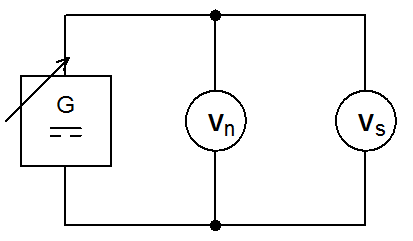
\includegraphics[scale=0.7]{schema.png}
\caption{Schéma zapojení}
\end{figure}

\section{Postup měření}
Obvod se zapojí dle schématu. Daný rozsah se rozdělí na cca 10 stejných intervalů (význačných hodnot celého rozsahu např. po deseti dílcích při ověřování rozsahu s desítkovou stupnicí). Před připojením napájecího napětí se zkontroluje nula přístroje. Popř. se nula dostaví pomocí nulovacího ústrojí.

Zvolené hodnoty se nastavují na ověřovaném přístroji a skutečná napětí pak odečítají
z normálového voltmetru. Pro vymezení tření v ložiskách elektromechanického přístroje se
měření provádí dvakrát (ve směru zvětšování napětí a ve směru dolů). Při nastavování hodnot je třeba dbát, abychom nastavovanou hodnotu nepřesáhli a nevraceli se z druhé strany.V takovém případě je nutné vrátit se o delší úsek stupnice a najíždět na nastavovanou hodnotu znova.

\section{Naměřené a dopočítané hodnoty}
Hodnoty počítáme dosazením do níže uvedených vzorců.
\captionof{table}{Naměřené a dopočítané hodnoty}
\begin{tabular}{|c|c|c|c|c|c|c|c|c|c|c|}
\hline 
$U_N[V]$ & 1,5 & 3 & 4,5 & 6 & 7,5 & 9 & 10,5 & 12 & 13,5 & 15 \\ 
\hline 
$\alpha [d]$ & 15 & 30 & 45 & 60 & 75 & 90 & 105 & 120 & 135 & 150 \\ 
\hline 
$k[V/d]$ & 0,1 & 0,1 & 0,1 & 0,1 & 0,1 & 0,1 & 0,1 & 0,1 & 0,1 & 0,1 \\ 
\hline 
$U_{S+}[V]$ & 1,530 & 2,946 & 4,497 & 5,984 & 7,458 & 8,969 & 10,459 & 11,940 & 13,431 & 14,930 \\ 
\hline 
$U_{S-}[V]$ & 1,519 & 2,990 & 4,510 & 6,004 & 7,486 & 8,972 & 10,468 & 11,933 & 13,450 & 14,930 \\ 
\hline 
$U_S[V]$ & 1,525 & 2,968 & 4,504 & 5,994 & 7,472 & 8,971 & 10,464 & 11,937 & 13,441 & 14,930 \\ 
\hline 
$K[V]$ & 0,025 & -0,032 & 0,004 & -0,006 & -0,028 & 0,029 & -0,036 & -0,063 & -0,059 & -0,070 \\ 
\hline 
\end{tabular} 
\\[0.5cm]

Kde $U_N$ je nastavovaná hodnota, $\alpha$  je výchylka cejchovaného měřidla, v dílcích stupnice, $k$ je konstanta cejchovaného měřidla, $U_{S+}$ je skutečná hodnota, napětí změřené normálem ve směru nahoru, $U_{S-}$ je skutečná hodnota, napětí změřené normálem ve směru dolů, $U_S$ je aritmetický průměr hodnot $U_{S+}$ a $U_{S-}$ a $K$ je korekce.

Pro výpočty použijeme následující vzorce:

Aritmetický průměr hodnot $U_{S+}$ a $U_{S-}$:
\begin{equation}
U_S = \frac{U_{S+}+U_{S-}}{2} = \frac{1,530+1,525}{2} = 1,525V
\end{equation}

Korekce:
\begin{equation}
K = U_S - U_N = 1,525-1,5 = 0,025V
\end{equation}

Třída přesnosti:
\begin{equation}
t_p = \frac{|\Delta _{max}|}{M}\cdot 100 = \frac{|-0,07|}{15}\cdot 100=0,467
\end{equation}
Předložený voltmetr měl však třídu přesnosti 0,2, tzn. že voltmetr již nevyhovuje původní třídě přesnosti.

\section{Grafy}
\begin{figure}[H]
\centering
	\begin{tikzpicture}
		\begin{axis}[
			width=1\textwidth,
	      	height=0.5\textwidth,
			xlabel={$U_N[V]$},
			ylabel={$K[V]$}]
		\addplot[color=red,mark=x] coordinates {
			(1.50,0.025)
			(3.00,-0.032)
			(4.50,0.004)
			(6.00,-0.006)
			(7.50,-0.028)
			(9.00,0.029)
			(10.5,-0.036)
			(12.0,-0.063)
			(13.5,-0.059)
			(15.0,-0.070)
		};
		\addlegendentry{$K=f(U_N)$}
		\addplot[color=blue,dashed] coordinates {
			(1.50,0)
			(15.0,0)
		};
		\addlegendentry{ideální}
		\end{axis}
	\end{tikzpicture}
	\caption{Korekční křivka}
\end{figure}

\section{Závěr}
Třída přesnosti cejchovaného přístroje je podle největší výchylky větší, než deklarovaná třída přesnosti stanovená na jeho stupnici. Z toho plyne, že cejchovaný přístroj již této třídě přesnosti \textbf{nevyhovuje}. Přístroj patří do třídy přesnosti $0,5$. Jinak je mechanický stav přístroje na první pohled v dobrém stavu.

\section{Přístroje}
\begin{itemize}
\item Cejchovaný voltmetr VLI-31/5, ML20, rozsah 0-15V
\item Normálový multimetr Agilent 34405A, ev. 206131
\item Regulovatelný zdroj Agilent E3610A, ev. 207512
\end{itemize}

\end{document}
